\chapter{Processing Models}

\section{Motivation}
\begin{definitionbox}{Processing Model}
    A mechanism used to connect operators acting on data in a query.
    \begin{itemize}
        \item Choice is critical to database design.
    \end{itemize}
\end{definitionbox}

\begin{definitionbox}{Function Objects}
    References to code that can be passed, invoked, change state and produce values.
    \begin{minted}{cpp}
#include <functional>

std::function<int(int, int)> add = [ /* captures */ ](int a, int b) { return a + b; }
    \end{minted}
    See \href{https://en.cppreference.com/w/cpp/language/lambda}{C++11 Lambdas}
    \begin{itemize}
        \item Can capture variables (value and references to) (also called closures).
        \item Used to implement single abstract method classes in some languages (e.g kotlin, java)
    \end{itemize}
\end{definitionbox}

\section{Volcano Processing}
\begin{definitionbox}{Volcano Processing Model}
    \begin{center}
        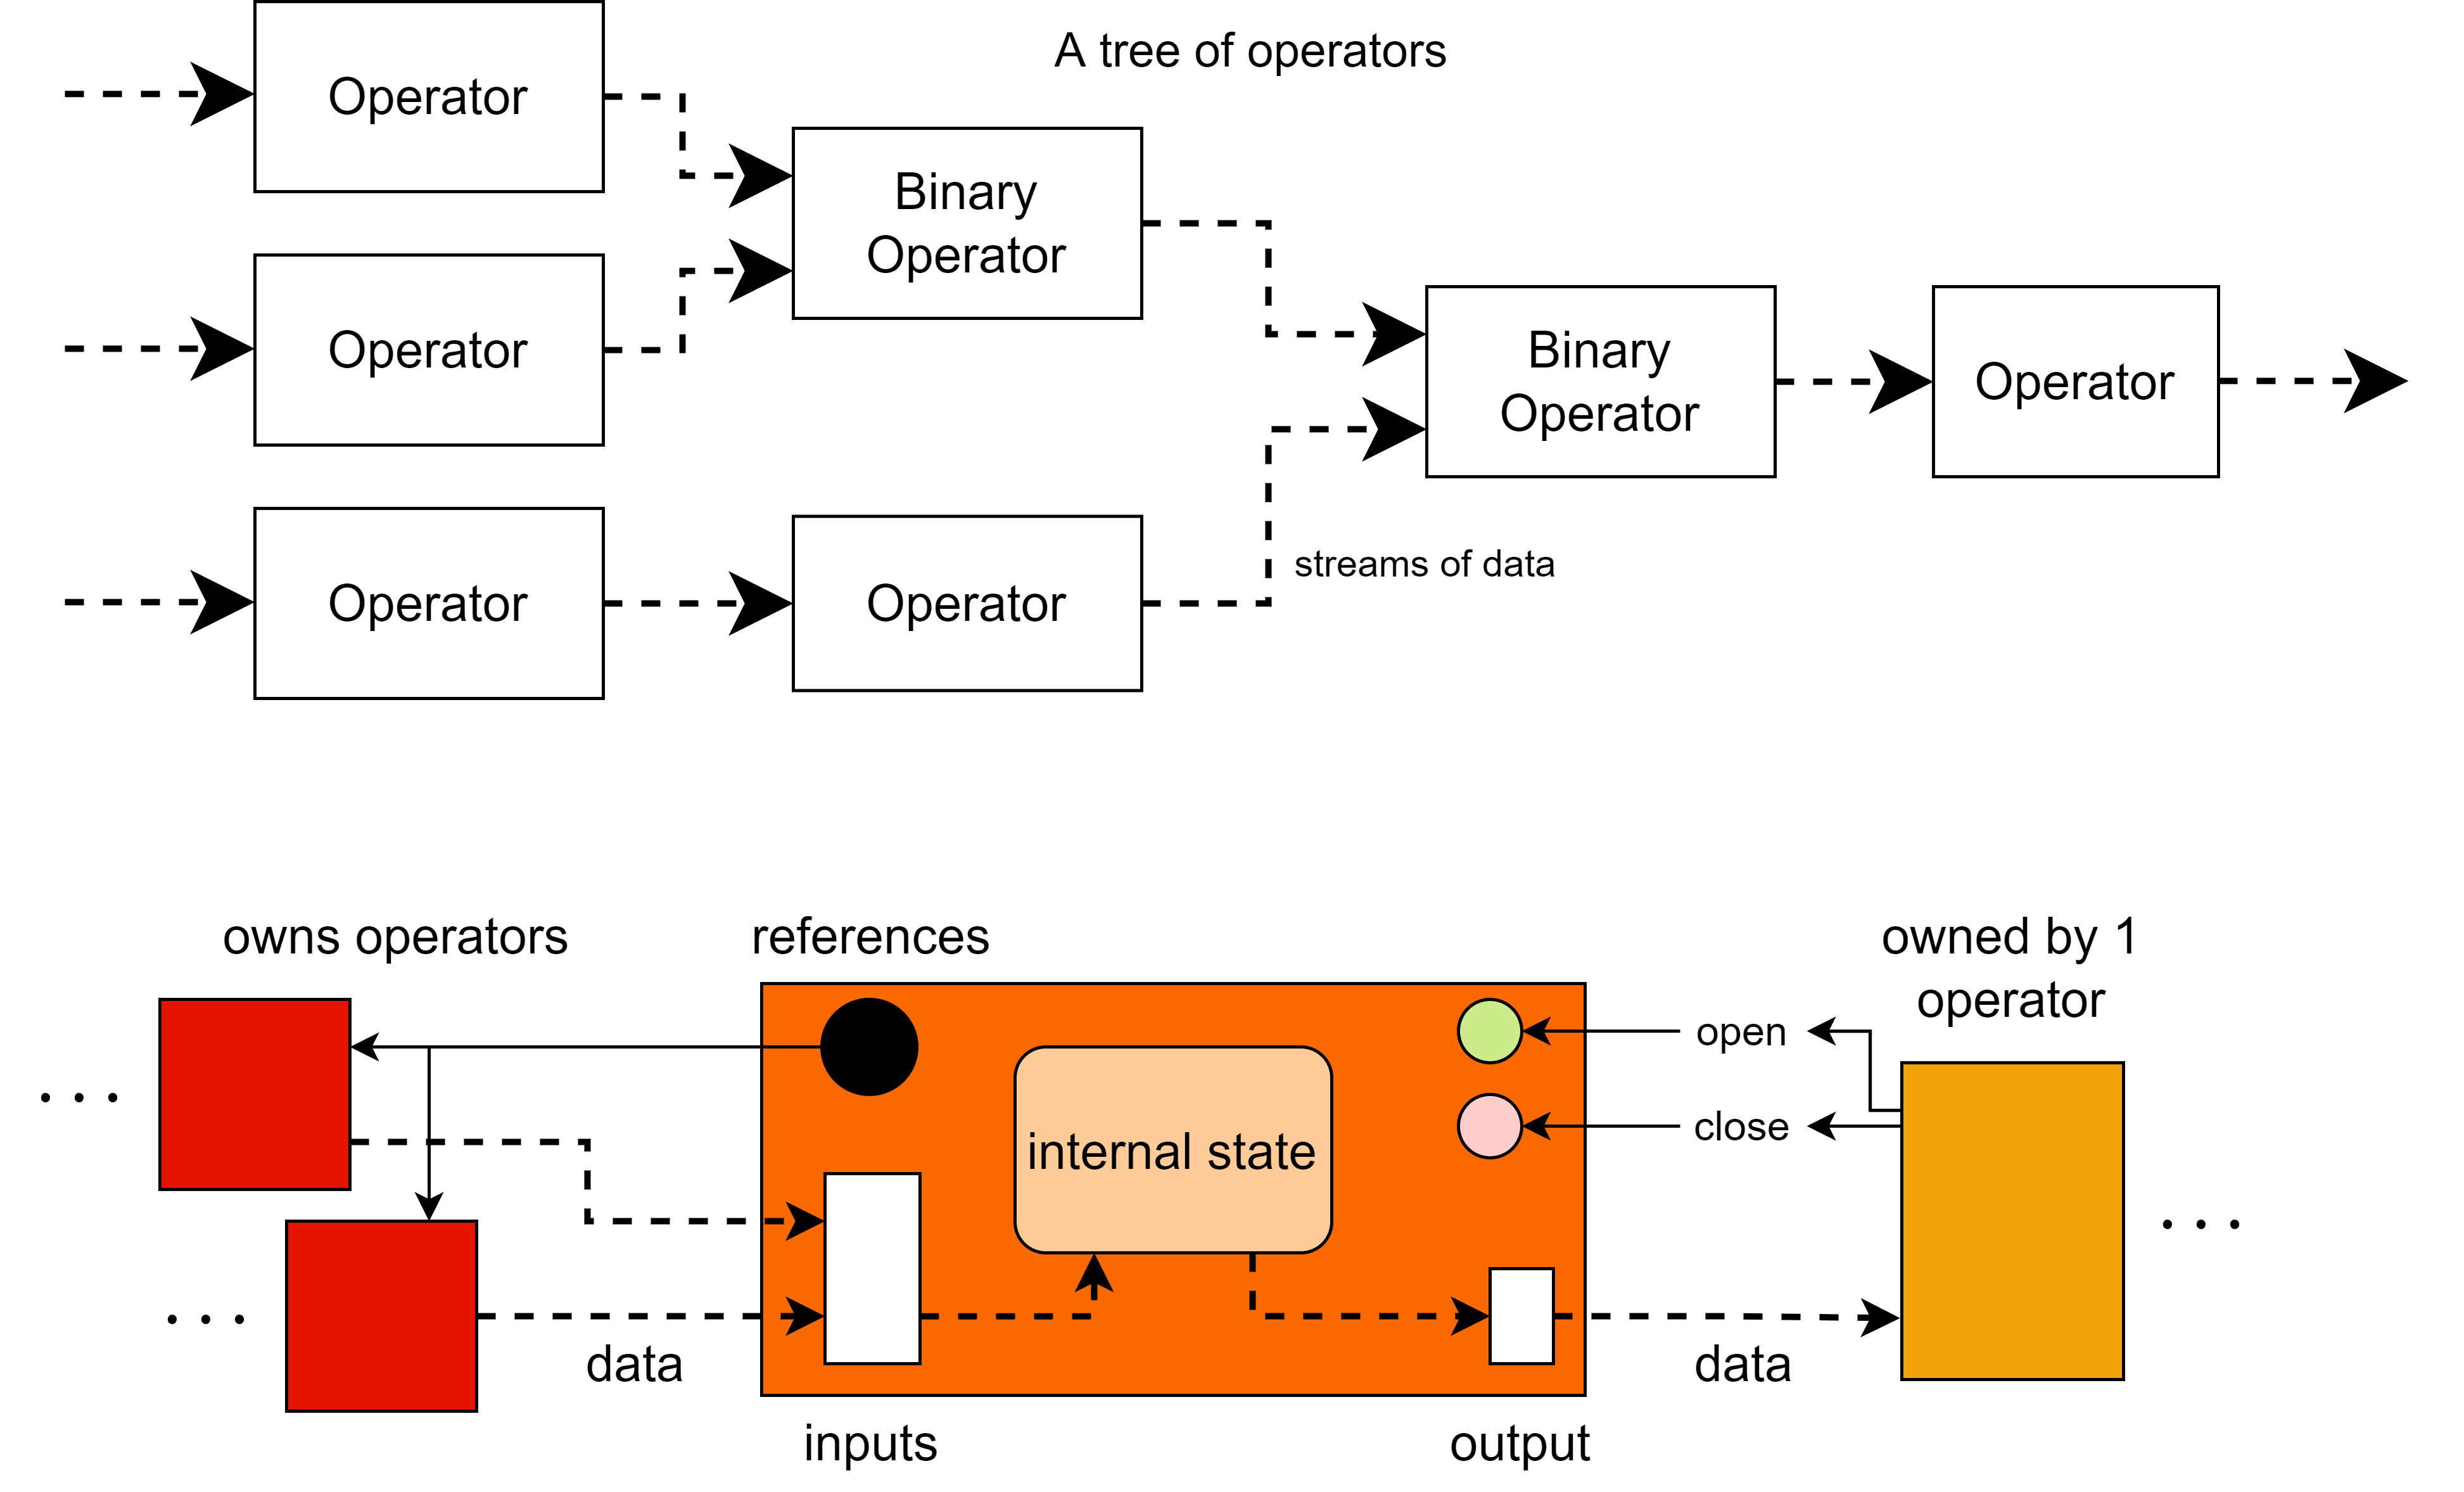
\includegraphics[width=.9\textwidth]{processing_models/images/volcano_stages.drawio.png}
    \end{center}
    Data is fed chunk by chunk (row) through a tree of operators.
    \begin{itemize}
        \item Older design (influential in the 80s) with a focus on design practices over performance. At the time this was an alternative to ad-hoc implementation.
        \item Uses non-relational physical algebra (specialized to be useful in expressing queries for a physical plan, rather than as an abstraction for the programmer).
    \end{itemize}
\end{definitionbox}

\subsection{Operators}
A basic interface for operators can be devised as:
\begin{minted}{cpp}
template <typename T>
struct Operator
{
  virtual void open() = 0;
  virtual void close() = 0;
  virtual optional<T> next() = 0;
};
\end{minted}
In order to allow the greatest flexibility in using our operators, they are parameterised by \mintinline{cpp}{typename T}. 
In the concrete examples this is set as a \textit{runtime tracked} type \mintinline{cpp}{Row} which is variable size, and contains variants of \mintinline{cpp}{int}, \mintinline{cpp}{char}, \mintinline{cpp}{bool}, etc.
\\
\\ We could also swap this out for a reference, or pointer to some \textit{runtime type} to avoid copying.

\begin{sidenotebox}{But why not RAII}
    To keep these examples explicit, an \mintinline{cpp}{open()} and \mintinline{cpp}{close()} are overriden, rather than using the constructor \& destructor.
    \\
    \\ That said RAII would be useful here:
    \begin{itemize}
        \item Automatically clean up after operators after they are dropped.
        \item Cannot be used before open/construction, or used after close/destruction.
    \end{itemize}
\end{sidenotebox}

\subsubsection{Scan}
Scans a table already loaded into memory to return its rows.
\begin{minted}{cpp}
template <typename T>
struct Scan : Operator<T>
{
  using TableType = vector<T>;
  /* Many different operators can have a reference to and read the table.
   * - shared_ptr drops table after it is no longer needed
   * - must avoid copying very large table structure
   */
  Scan(shared_ptr<TableType> t) : _table(t), _index(0) { assert(_table); }

  /* No operation on open / close */
  void open() override {}
  void close() override {}

  optional<T> next() override
  {
    if (_index < (*_table).size())
    {
      return (*_table)[_index++];
    }
    else
    {
      return {};
    }
  }

private:
  shared_ptr<TableType> _table;
  size_t _index;
};
\end{minted}

\subsubsection{Project}
\begin{minted}{cpp}
template <typename T, typename S>
struct Project : Operator<T>
{
  using Projection = function<T(S)>;

  Project(unique_ptr<Operator<S>> child, Projection proj)
      : _child(move(child)), _proj(proj)
  {
    assert(_child);
  }

  void open() override { _child->open(); }
  void close() override { _child->close(); }

  optional<T> next() override
  {
    // Note: can be simplified with optional<A>::and_then(function<B(A)>) in C++23
    auto next = _child->next();
    if (next.has_value())
    {
      return _proj(next.value());
    }
    else
    {
      return {};
    }
  }

private:
  unique_ptr<Operator<S>> _child;
  Projection _proj;
};
\end{minted}

\subsubsection{Select}
\begin{minted}{cpp}
template <typename T>
struct Select : Operator<T>
{
  using Predicate = function<bool(T)>;

  Select(unique_ptr<Operator<T>> child, Predicate pred)
      : _child(move(child)), _pred(pred)
  {
    assert(_child);
  }

  void open() override { _child->open(); }
  void close() override { _child->close(); }

  optional<T> next() override
  {
    auto candidate = _child->next();
    // keep getting candidates until there are no more, or one is valid.
    while (candidate.has_value() && !_pred(candidate.value()))
    {
      candidate = _child->next();
    }
    return candidate;
  }

private:
  unique_ptr<Operator<T>> _child;
  Predicate _pred;
};
\end{minted}

\subsubsection{Union}
\begin{minted}{cpp}
template <typename T>
struct Union : Operator<T>
{
  Union(unique_ptr<Operator<T>> leftChild, unique_ptr<Operator<T>> rightChild)
      : _leftChild(move(leftChild)), _rightChild(move(rightChild))
  {
    assert(_leftChild && _rightChild);
  }

  void open() override
  {
    _leftChild->open();
    _rightChild->open();
  }
  void close() override
  {
    _leftChild->close();
    _rightChild->close();
  }

  optional<T> next() override
  {
    auto candidate = _leftChild->next();
    if (candidate.has_value())
    {
      return candidate;
    }
    else
    {
      return _rightChild->next();
    }
  }

private:
  unique_ptr<Operator<T>> _leftChild, _rightChild;
};
\end{minted}

\subsubsection{Difference}

\begin{definitionbox}{Pipeline Breaker}
    An operator which can only produce its first value/output tuple after all inputs from one or more input operators has been processed.
    \begin{itemize}
        \item Usually requires some kind of buffering (e.g with \mintinline{cpp}{Difference}).
    \end{itemize}
\end{definitionbox}

Difference breaks the pipeline as we need to know all tuples from one side (the subtracting set) before we can start to produce rows.

\begin{minted}{cpp}
/* The definition of difference forces the pipeline to be broken (buffering) */
template <typename T>
struct Difference : Operator<T>
{
  Difference(unique_ptr<Operator<T>> fromChild,
             unique_ptr<Operator<T>> subChild)
      : _fromChild(fromChild), _subChild(subChild), _subBuffer()
  {
    assert(_fromChild && _subChild);
  }

  void open() override
  {
    _fromChild->open();
    _subChild->open();

    // buffer all to subtract
    for (auto candidate = _subChild->next(); candidate.has_value();
         candidate = _subChild->next())
    {
      _subBuffer.push_back(candidate);
    }
  }
  void close() override
  {
    _fromChild->close();
    _subChild->close();
  }

  optional<T> next() override
  {
    auto candidate = _fromChild->next();
    // keep getting next until there is no next candidate, or the candidate is
    // not being subtracted
    while (candidate.has_value() && _subBuffer.contains(candidate.value()))
    {
      candidate = _fromChild->next();
    }
    return candidate;
  }

private:
  unique_ptr<Operator<T>> _fromChild, _subChild;
  unordered_set<T> _subBuffer;
};
\end{minted}

\subsubsection{Cartesian/Cross Product}
This can be optionally implemented as a \textit{pipeline breaker}.

\begin{minted}{cpp}

template <typename A, typename B>
struct BreakingCrossProduct : Operator<tuple<A, B>>
{
  BreakingCrossProduct(unique_ptr<Operator<A>> leftChild,
                       unique_ptr<Operator<B>> rightChild)
      : _leftChild(move(leftChild)), _rightChild(move(rightChild)),
        _leftCurrent(), _rightIndex(0), _rightBuffer()
  {
    assert(_leftChild && _rightChild);
  }

  void open() override
  {
    _leftChild->open();
    _rightChild->open();

    // set first left (can be none -> in which case next will never return
    // anything)
    _leftCurrent = _leftChild->next();

    // buffer in the entirety of the right
    for (auto candidate = _rightChild->next(); candidate.has_value();
         candidate = _rightChild->next())
    {
      _rightBuffer.push_back(candidate.value());
    }
  }

  void close() override
  {
    _leftChild->close();
    _rightChild->close();
  }

  optional<tuple<A, B>> next() override
  {
    // invariant: _rightBuffer.size() > _rightIndex >= 0
    if (_leftCurrent.has_value() && !_rightBuffer.empty())
    {
      auto next_val =
          make_tuple(_leftCurrent.value(), _rightBuffer[_rightIndex]);

      _rightIndex++;
      if (_rightIndex == _rightBuffer.size())
      {
        _rightIndex = 0;
        _leftCurrent = _leftChild->next();
      }

      return next_val;
    }
    else
    {
      return {};
    }
  }

private:
  unique_ptr<Operator<A>> _leftChild;
  unique_ptr<Operator<B>> _rightChild;
  optional<A> _leftCurrent;
  size_t _rightIndex;
  vector<B> _rightBuffer;
};
\end{minted}
A Non-pipeline breaking implementation has two phases:
\begin{enumerate}
    \item Collecting rows from the right child operator, while using the same row from the left.
    \item The right child operator has been exhausted, slowly get tuples from the left while traversing tuples collected from the right.
\end{enumerate}
\begin{minted}{cpp}
template <typename A, typename B>
struct CrossProduct : Operator<tuple<A, B>>
{
  CrossProduct(unique_ptr<Operator<A>> leftChild,
               unique_ptr<Operator<B>> rightChild)
      : _leftChild(move(leftChild)), _rightChild(move(rightChild)),
        _leftCurrent(), _rightBuffered(), _rightOffset(0)
  {
    assert(_leftChild && _rightChild);
  }

  void open() override
  {
    _leftChild->open();
    _rightChild->open();
    _leftCurrent = _leftChild->next();
  }
  void close() override
  {
    _leftChild->close();
    _rightChild->close();
  }

  optional<tuple<A, B>> next() override
  {
    /* invariants:
     * - _leftCurrent is already set
     * - if there are no more _rightChild to get, then we are iterating over the
     *   _leftChild
     */
    auto rightCandidate = _rightChild->next();
    if (rightCandidate.has_value())
    {
      // still getting content from the right had side
      _rightBuffered.push_back(rightCandidate.value());
    }
    else if (_rightOffset == _rightBuffered.size())
    {
      // all tuples have been taken from right hand side, now using buffer
      _leftCurrent = _leftChild->next();
      _rightOffset = 0;
    }

    // only return if both sides have values
    if (_leftCurrent.has_value() && !_rightBuffered.empty())
    {
      // get tuple and increment _rightOffset
      return make_tuple(_leftCurrent.value(), _rightBuffered[_rightOffset++]);
    }
    else
    {
      return {};
    }
  }

private:
  unique_ptr<Operator<A>> _leftChild;
  unique_ptr<Operator<B>> _rightChild;
  optional<A> _leftCurrent;
  vector<B> _rightBuffered;
  size_t _rightOffset;
};
\end{minted}

\subsubsection{Group Aggregation}
This is fundamentally a \textit{pipeline breaker}, and must buffer rows prior to \mintinline{cpp}{next()}. 
The algorithm acts in three phases:
\begin{enumerate}
    \item Buffer tuples from the child.
    \item Get the key (column being grouped by e.g \mintinline{SQL}{GROUP BY column1}) and aggregation (e.g \mintinline{SQL}{SELECT MAX(column2)}) and place in a hashmap.
    \item Finally provide rows through \mintinline{cpp}{next()}
\end{enumerate}
\begin{minted}{cpp}
/* We use the template to determine the hash and nextSlot implementations used
 * T        -> type of data provided by the child
 * S        -> data output by the groupBy & aggregation
 * K        -> the type grouped on, produced by a grouping function (K group(T))
 * hash     -> a function to convert a key into a hash
 * nextSlot -> to determine next slot in collisions
 */
 template <typename T, typename S, typename K, size_t nextSlot(size_t),
          size_t hashFun(K), size_t OVERALLOCATE_FACTOR = 2>
struct GroupBy : Operator<S>
{
  using Aggregation = function<S(optional<S>, T)>;
  using Grouping = function<K(T)>;

  GroupBy(unique_ptr<Operator<T>> child,
          Grouping grouping,
          Aggregation aggregation) : _child(move(child)), _grouping(grouping),
                                     _aggregation(aggregation), _hashTable(), _hashTableCursor(0)
  {
    assert(_child);
  }

  void open() override
  {
    _child->open();

    vector<T> childValues;
    for (auto currentVal = _child->next();
         currentVal.has_value();
         currentVal = _child->next())
    {
      childValues.push_back(currentVal.value());
    }

    _hashTable = vector<optional<pair<K, S>>>(childValues.size(), optional<pair<K, S>>());
    for (T val : childValues)
    {
      K key = _grouping(val);
      size_t slot = hashFun(key) % _hashTable.size();
      while (_hashTable[slot].has_value() && _hashTable[slot].value().first != key)
      {
        slot = nextSlot(slot) % _hashTable.size();
      }

      // slot is now correct, either a value present with the same key, or none.
      auto prev_val = _hashTable[slot].has_value() ? _hashTable[slot].value().second : optional<S>();
      _hashTable[slot] = optional<pair<K, S>>(make_pair<K, S>(move(key), _aggregation(prev_val, val)));
    }

    // all values moved into the hashtable, so vector deallocated
  }

  void close() override
  {
    _child->close();
  }

  optional<S> next() override
  {
    while (_hashTableCursor < _hashTable.size())
    {
      auto slot = _hashTable[_hashTableCursor];
      _hashTableCursor++;

      if (slot.has_value())
      {
        return slot.value().second;
      }
    }
    return {};
  }

private:
  Aggregation _aggregation;
  Grouping _grouping;
  unique_ptr<Operator<T>> _child;
  vector<optional<pair<K, S>>> _hashTable;
  size_t _hashTableCursor;
};
\end{minted}

\subsubsection{Operators Composed}
We can finally define types to use with our operators.
\begin{minted}{cpp}
using Value = variant<int, char, bool>;
using Row = vector<Value>;
using Table = vector<Row>;
\end{minted}
And now build a query from them
\begin{minted}{cpp}
SELECT table.1, MAX(table.0) FROM table GROUP BY table.1;
\end{minted}
\begin{minted}{cpp}
shared_ptr<Table> data = make_shared<Table>(Table{
    {1, 'c', true},
    {1, 'c', false},
    {2, 'c', false},
    {1, 'd', true},
    {3, 'e', false}});

auto scan1 = make_unique<Scan<Row>>(data);
auto scan2 = make_unique<Scan<Row>>(data);
auto cross = make_unique<CrossProduct<Row, Row>>(move(scan1), move(scan2));

Project<Row, tuple<Row, Row>> proj(move(cross), [](tuple<Row, Row> t)
                                    {
auto vec2 = get<1>(t);
auto vec1 = get<0>(t);
vec1.insert(vec1.end(), vec2.begin(), vec2.end());
return vec1; });

GroupBy<Row, Row, Value, nextSlotLinear, hashValue>
    groupby(move(scan), groupBySecondCol, aggregateSecondCol);

groupby.open();
for (auto val = groupby.next(); val.has_value(); val = groupby.next())
{
  cout << val.value() << endl;
}
groupby.close();
\end{minted}

\begin{minted}{bash}
[ 3 e]
[ 5 c]
[ 1 d]
\end{minted}

\begin{sidenotebox}{Run it!}
    The above code is provided with examples in the associated notes repository!
\end{sidenotebox}